\documentclass[12pt]{article}
\usepackage[landscape,a4paper,pdftex]{geometry}
\usepackage[english]{babel}
%\usepackage{fullpage}
\usepackage{amsmath,amssymb}
\usepackage{array}
\usepackage{graphicx}
\usepackage{wrapfig,color}
\usepackage{multirow}
\usepackage{rotating}
\usepackage{xspace}
\usepackage{pifont}
\usepackage{url}

%\setlength{\textwidth}{19cm}
%\setlength{\textheight}{26cm}
%\setlength{\voffset}{-2.6cm} % 2.6 for EPS, 1.0 for CPS
%\setlength{\hoffset}{-2.9cm}
%These are are for full landscape; use ``dvips -T 29.7cm,21cm ...''
%Also ... to get them a bit smaller for transparencies:
%    ``dvips -T 29.7cm,21cm -x 930 -O 1cm,0.6cm ...''
\setlength{\textwidth}{27cm}
\setlength{\textheight}{17.3cm}
\setlength{\voffset}{-4mm}
\setlength{\hoffset}{-15mm}

%\paperwidth=296mm
%\paperheight=210mm

\parindent=-5mm
\parskip=1mm
\parsep=0pt
\itemsep=-4mm
\topsep=0pt
\partopsep=0pt

\renewcommand{\floatpagefraction}{0.95}
\renewcommand{\topfraction}{0.9}
\renewcommand{\textfraction}{0.1}

\renewcommand{\thefootnote}{\fnsymbol{footnote}}
\renewcommand{\arraystretch}{0.9}

\definecolor{purple}{rgb}{0.5,0.2,0.6}
\definecolor{dred}{rgb}{0.3,0,0}
\definecolor{dblue}{rgb}{0,0,0.5}
\definecolor{dgreen}{rgb}{0,0.5,0}
\definecolor{dyellow}{rgb}{0.4,0.4,0}

\definecolor{freshcol}{rgb}{0.2,0.4,0.05}

\usepackage{fancyheadings}
\lhead{\sffamily Matev\v{z} Tadel}
\chead{\sffamily The basic concepts of \gled}
\rhead{\sffamily \thepage}
\lfoot{}
\cfoot{}
\rfoot{\sffamily ALICE Offline weekly, 7. October 2004}

\pagestyle{fancy}

\def\nl{\newline}
\def\ml{\medskip\hrule\medskip}
\def\bl{\bigskip\hrule\bigskip}
\def\hs6{\hbox to 6mm{}}
\def\q{\quad}
\def\qq{\quad\quad}
\def\bull{$\bullet$\hbox to 2mm{}}
\def\qtoq{\q$\to$\q}

\def\smalltt#1{{\large\texttt{#1}}}
\def\foottt#1{{\normalsize\texttt{#1}}}

\def\gled{\textsc{Gled}\xspace}
\def\p7{\texttt{project7}\xspace}
\def\grid{\texttt{grid}\xspace}
\def\root{\textsc{ROOT}\xspace}
\def\cint{\textsc{CINT}\xspace}
\def\rootcint{\texttt{rootcint}\xspace}
\def\cxx{\smalltt{C++}\xspace}

\def\iec{i.e.,\xspace}
\def\egc{e.g.,\xspace}
\def\ie{i.e.\xspace}
\def\eg{e.g.\xspace}

\def\MB{\,\rm{MB}}
\def\GB{\,\rm{GB}}
\def\TB{\,\rm{TB}}
\def\PB{\,\rm{PB}}
\def\Gbit{\,\rm{Gbit}}

\def\MHz{\,\rm{MHz}}
\def\kHz{\,\rm{kHz}}
\def\Hz{\,\rm{Hz}}

%%%%%%%%%%%%%%%%%%%%%%%%%%%%%%%%%%%%%%%%%%%%
% Local

\def\gledihscmdir{../../papers/gled-ihscm}
\def\gledauthdir{../../papers/gled-auth}

\begin{document}
%\psdraft
\sffamily\Large

%%%%%%%%%%%%%%%%%%%%%%%%%%%%%%%%%%%%%%%%%%%%
% Frontpage
\thispagestyle{empty}

\centerline{\Huge The basic concepts of \gled}
\bigskip
\centerline{\texttt{matevz.tadel@gled.org}}
\medskip
\centerline{\color{dred}\url{http://www.gled.org/} \qq 
  \color{dgreen}\url{http://gled.ijs.si/}}

\vskip 8mm

\textbf{\gled is} a \cxx framework/toolkit, heavily based on
\root, and having much the same flavour

\begin{enumerate}
\item distributed computing (hierarchical server-client model)%
  \hfill {\large really too early to say more}

\item management of object collections and object-interaction (w/GUI)%
  \hfill {\large (1) $\to$ collaborative tools}

\item dynamic 3D visualization (OpenGL)%
  \hfill {\large (1\&2) $\to$ multiplayer online game engine}
\end{enumerate}

\medskip
\centerline{{\color{dblue}\texttt{GLED -- Generick Lightweight Environment for Distributed computing}}}
\bigskip

\textbf{History:} proto-implementation 1998 (not much of the code left)\nl
used it in 2000 for analysis, simulation and visualiztion of a
test-beam set-up\nl
since mid 2001 working on it $\sim 70\%$

first public release \texttt{gled-1.2.0} in June 2003\nl
1.2.3 released this June

altogether $\sim4.5$\;work-years; (S)F support provided by J. Javor\v{s}ek

last half year actually being used for steering and visualization of
\texttt{Pythia6} extended with user-processes

\bigskip

\textbf{Availability:} \texttt{GNU/Linux}, but no general reason
against portability\hfill \textbf{License:} GPL-2.0

\newpage
\setcounter{page}{1}
%%%%%%%%%%%%%%%%%%%%%%%%%%%%%%%%%%%%%%%%%%%%%%%%%%%%%%%%%%%%%%%%%%%%%%%%
% ROOT as a base framework

\textbf{\LARGE \root, from the perspective of \gled, has:} 

\bigskip
\textbf{Versatile object serialization methods and
  accompanying services}\nl
%
inner file structure w/versioning: \texttt{TFile \& TDirectory}\nl
%
\texttt{rootd}: such service absolutely necessary for a distributed
system\nl
%
object aggregation methods: \texttt{C}-pointers, \texttt{TRef} and
\texttt{TCollection}\nl
%
\hs6 (in fact \gled also uses some of its own; but \root offers a very
clean data model)

\bigskip
\textbf{Good (and portable) OS interface}\qq (would need some
modularization in appl. start-up \& event handling)\nl
networking \dots\ in future use also authentication and (optionally)
\texttt{TSecureSocket}\nl
thread abstraction layer (khm \dots\ actually \gled uses its own
\texttt{pthread} wrapper classes)

\bigskip
\textbf{A most complete set of data-analysis \& scientific
  visualization elements}\nl
histograms for displaying server monitoring statistcs (could be
trees)\nl
linear algebra package for 3D geometry

\bigskip
\textbf{Introspection \& user-interaction bindings ---
  \texttt{TClass}, \cint \&
  \rootcint}\nl
introspection \q$\to$\q streaming, on-line object interaction, dynamic
GUI\nl
start-up scripts; excellent as application configuration and start-up steering

But there is some pain w/\cint:\nl
interwoven w/\root as application framework (streaming, GUI)\nl
fault tolerance could be better (nothing critical, but affects \root
as application)\nl
thread safety\nl
impossible to prevent object-access to the user (locking, remote
method execution)

\newpage
%%%%%%%%%%%%%%%%%%%%%%%%%%%%%%%%%%%%%%%%%%%%%%%%%%%%%%%%%%%%%%%%%%%%%%%%
% Gled preface ... the base class ZGlass

\textbf{\LARGE \gled as a \texttt{C++} framework/toolkit w/strong {\root}s} 

\bigskip
\textbf{Any OO framework/toolkit is all about objects and classes,}
but in particular:
\hfill{{\color{dgreen} \large GUI, visualization}\qq}
\nl
%
A) What you can do w/them? [data access, method execution, object
structuring, alternative representations]\nl
%
B) What they can do for you? [application functionality]

\bigskip
\textbf{\eg \root:}\qq \texttt{TObject} class offers serialization and introspection
methods\nl
coupled w/\root as an application you get: interactive access, object
browsing/GUI, \texttt{Draw()} into \texttt{TPad}

\bl

\textbf{Base-class for fully enabled \gled objects:} \qq \texttt{class ZGlass :
public TObject \dots}
\begin{enumerate}
  
\item method call serialization \& execution: \qq\qq {\color{dblue}\texttt{MIR --
    Method Invocation Request}}\nl
%
  \texttt{class ZMIR : public TMessage \q \dots} \hfill includes routing \&
  caller information, possibly a result request\nl
%
  execution of MIRs carried out by {\color{dblue}\emph{lenses}}
  themselves;\hfill in \gled as appl.\ steered and aided by other services
  
\item automatic generation of remote-execution methods, the per-class
  \texttt{MIR} execution code and \texttt{Get/Set} methods\nl
%
  \eg \texttt{void ClassX::DoSomething(args)} $\to$ \texttt{ZMIR*
    ClassX::{\color{red}S\_}DoSomething(args)} \nl
%
  accepts also \texttt{TObject}s as arguments and can hold arbitrary `data
  tail' (can be used for data transfer!)\nl
%
  the \texttt{Set} methods also have \texttt{S\_Set} counterparts \q
  $\to$ \q natural means for object-data synchronization

\item object aggregation methods (called links and lists) \hfill %
  must survive in a distributed environment!
  
\item reference counting w/ optional reverse-referencing

\item locking with granularity on per-object level \hfill (this is perhaps
  too strong)

\end{enumerate}
Glasses much more heavyweight: \smalltt{\color{dred}sizeof(TObject)=12,
  sizeof(ZGlass)=128; \qq sizeof(TNamed)=28.}

\newpage
%%%%%%%%%%%%%%%%%%%%%%%%%%%%%%%%%%%%%%%%%%%%%%%%%%%%%%%%%%%%%%%%%%%%%%%%
% Lens habitat, HSCM, Kings\&Queens

{\LARGE\textbf{Lens habitat:} a hierarchic server-client model}
\bigskip

\hbox to \hsize{%
  \vbox{\hsize=18cm%
    
    Arbitrary tree-graph of \gled application instances (\gled-nodes)
    forming a \gled-cluster (or better a \gled-tree); connected via
    TCP sockets
    
    A general node is a client, server and a proxy \q $\Rightarrow$ \q
    \textbf{\color{dblue}Saturn}

    Lenses populate \emph{lens-spaces} on Saturns:
    \smallskip

    \vbox{\normalsize\baselineskip=-\maxdimen\lineskiplimit=\maxdimen\lineskip=6pt
      \noindent
      \hbox to 3cm{\color{dyellow} sun-space:} server\nl
      \hbox to 3cm{\color{dgreen} moon-space:} client/proxy\nl
      \hbox to 3cm{\color{dred} fire-space:}   local stuff;
      computation, GUI representation/control, visualization (trinagulations)
     }

    Saturn accepts connections from client Saturns or Eyes (local
    viewers)\nl
    represented by glasses \texttt{SaturnInfo}\&\texttt{EyeInfo}
    (stored on SunAbsolute)\nl
    {\color{dred}\gled-cluster structure available from within \gled!}

    To request a method execution, a MIR is passed to a Saturn,
    \eg:{\large\begin{verbatim}
auto_ptr<ZMIR> mir( lens->S_SomeMethod(args) );
saturn->ShootMir(mir);                    // ASync
ZMIR_RR* saturn->ShootMIRWaitResult(mir); //  Sync
\end{verbatim}
  }
}
  \hss
  \vbox{\hsize=7cm%
    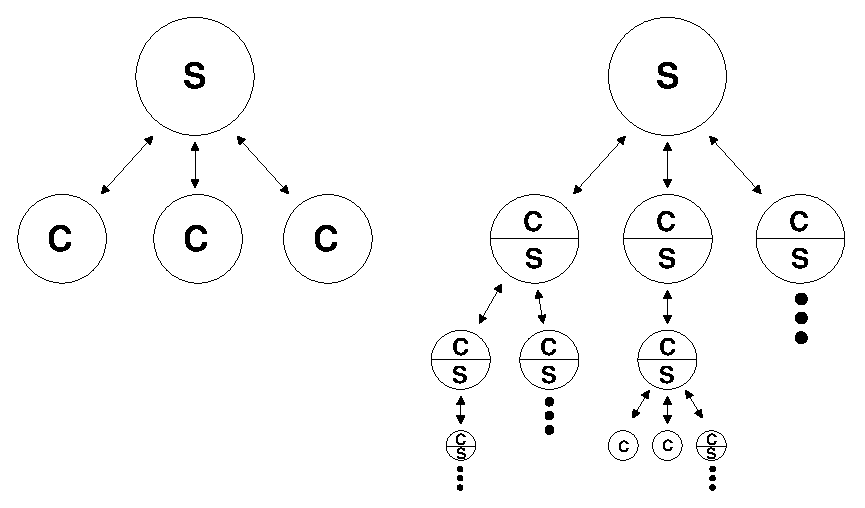
\includegraphics[width=\hsize]{\gledihscmdir/figs/hscm}
    \vskip 5mm
    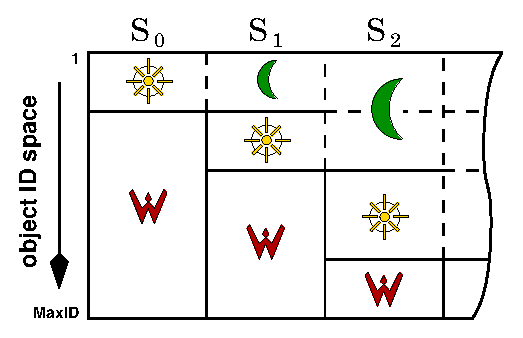
\includegraphics[width=\hsize]{\gledihscmdir/figs/ID_space}
    %\vskip 15mm
  }
}

\texttt{\large\color{dblue}class ZMIR\_RR : public TBuffer} \qtoq
{\color{dred}Any data can be returned!}\hfill
\texttt{\normalsize typedef ZMIR\_Result\_Report ZMIR\_RR;}

\bl

Saturn is a complex MIR router and execution environment,
supporting:\begin{itemize}\itemsep=-1mm
\item {\color{dblue}Flared} (broadcast) and {\color{dblue}Beamed} (directed)
MIR routing

\item ASync.\&Sync. MIR execution \hfill {\color{dblue}but one should
    know what he's doing in Sync.\ mode}

\item Detached Flare and Beam execution: Saturn spawns a new thread
  for the method call

\item Delayed MIR execution (like \texttt{'at'} command)

\end{itemize}

\newpage
%%%%%%%%%%%%%%%%%%%%%%%%%%%%%%%%%%%%%%%%%%%%%%%%%%%%%%%%%%%%%%%%%%%%%%%%
% Kings, Queens; Lens life-span \& auth intro

\textbf{\LARGE Rulers of lens-spaces (Kings) and rulers of lenses (Queens)}
\bigskip

\hbox to \hsize{%
  \vbox{\hsize=22cm%
    Each Saturn-level lens-space is ruled by a 
    glass \texttt{ZKing}\nl
    mostly administrative entity \q $\to$ \q allocation of
    {\color{dblue}queen-spaces}\nl
    aids during Queen mirroring (by using Eunuchs)

    Queens (glass \texttt{ZQueen}) are the true rulers of lenses:\nl
    \bull take care of instantiation and deletion of lenses +
    ref.\ counting \& garbage collection\nl
    \bull \texttt{BlessMIR}s targeted at their subjects: dependency checking
    \& user authorization\nl
    \bull they are the smallest unit mirrored independently to moons\nl
    \bull they hold a list of queens they depend on:\nl
    \hs6 if $q$ depends on $q'$ $\Rightarrow$ lenses of $q$ can
    reference lenses of $q'$ and receive them as MIR args\nl
    \bull sub-classes of \texttt{ZQueen}: have \texttt{ZSunQueen}\hfill
    \hs6 {\color{dblue}could have \texttt{RootFileQueen},
      \texttt{SqlQueen}, \dots}
  }
  \hss
  \vbox{\hsize=4cm%
    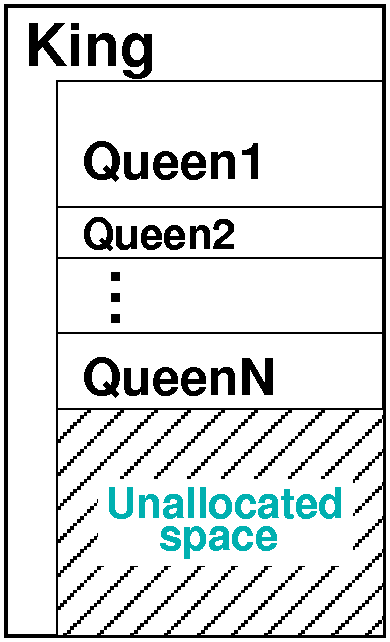
\includegraphics[width=\hsize]{king-queens}
    \vskip 5mm
  }
}

\bl

\textbf{\LARGE MIR filtering --- core MIR exexution authorization mechanism}
\bigskip

After dependency check queen consults the relevant {\color{dblue}MIR
  filters}:\nl
  a) \hbox to 9cm{\texttt{\large\color{dblue}ZMirFilter* ZGlass::mGuard}}%
    per lens filter (of course, many lenses can share the same filter)\nl
  b) \hbox to 9cm{\texttt{\large\color{dblue}ZMirFilter* ZQueen::mProtector}}%
  filter protecting all subjects of a queen

Either of the two or both filters can be used, depending on queen settings:\nl
{\large\verb!enum ZQueen::AuthMode_e { AM_None=0, AM_Queen, AM_Lens, AM_QueenThenLens, AM_LensThenQueen };!}

MIR filters can be aggregated: %
{\large\color{dblue}\verb!class ZFilterAggregator : public ZMirFilter!}\nl
  arbitrarily complex authorization rules can be constructed \hfill%
  {\large\color{dred}(and, of course, shared by many lenses/queens!)}

Concept of a user is split into: Identity and MirEmittingEntity

\newpage
%%%%%%%%%%%%%%%%%%%%%%%%%%%%%%%%%%%%%%%%%%%%%%%%%%%%%%%%%%%%%%%%%%%%%%%%
% Authorization details

\centerline{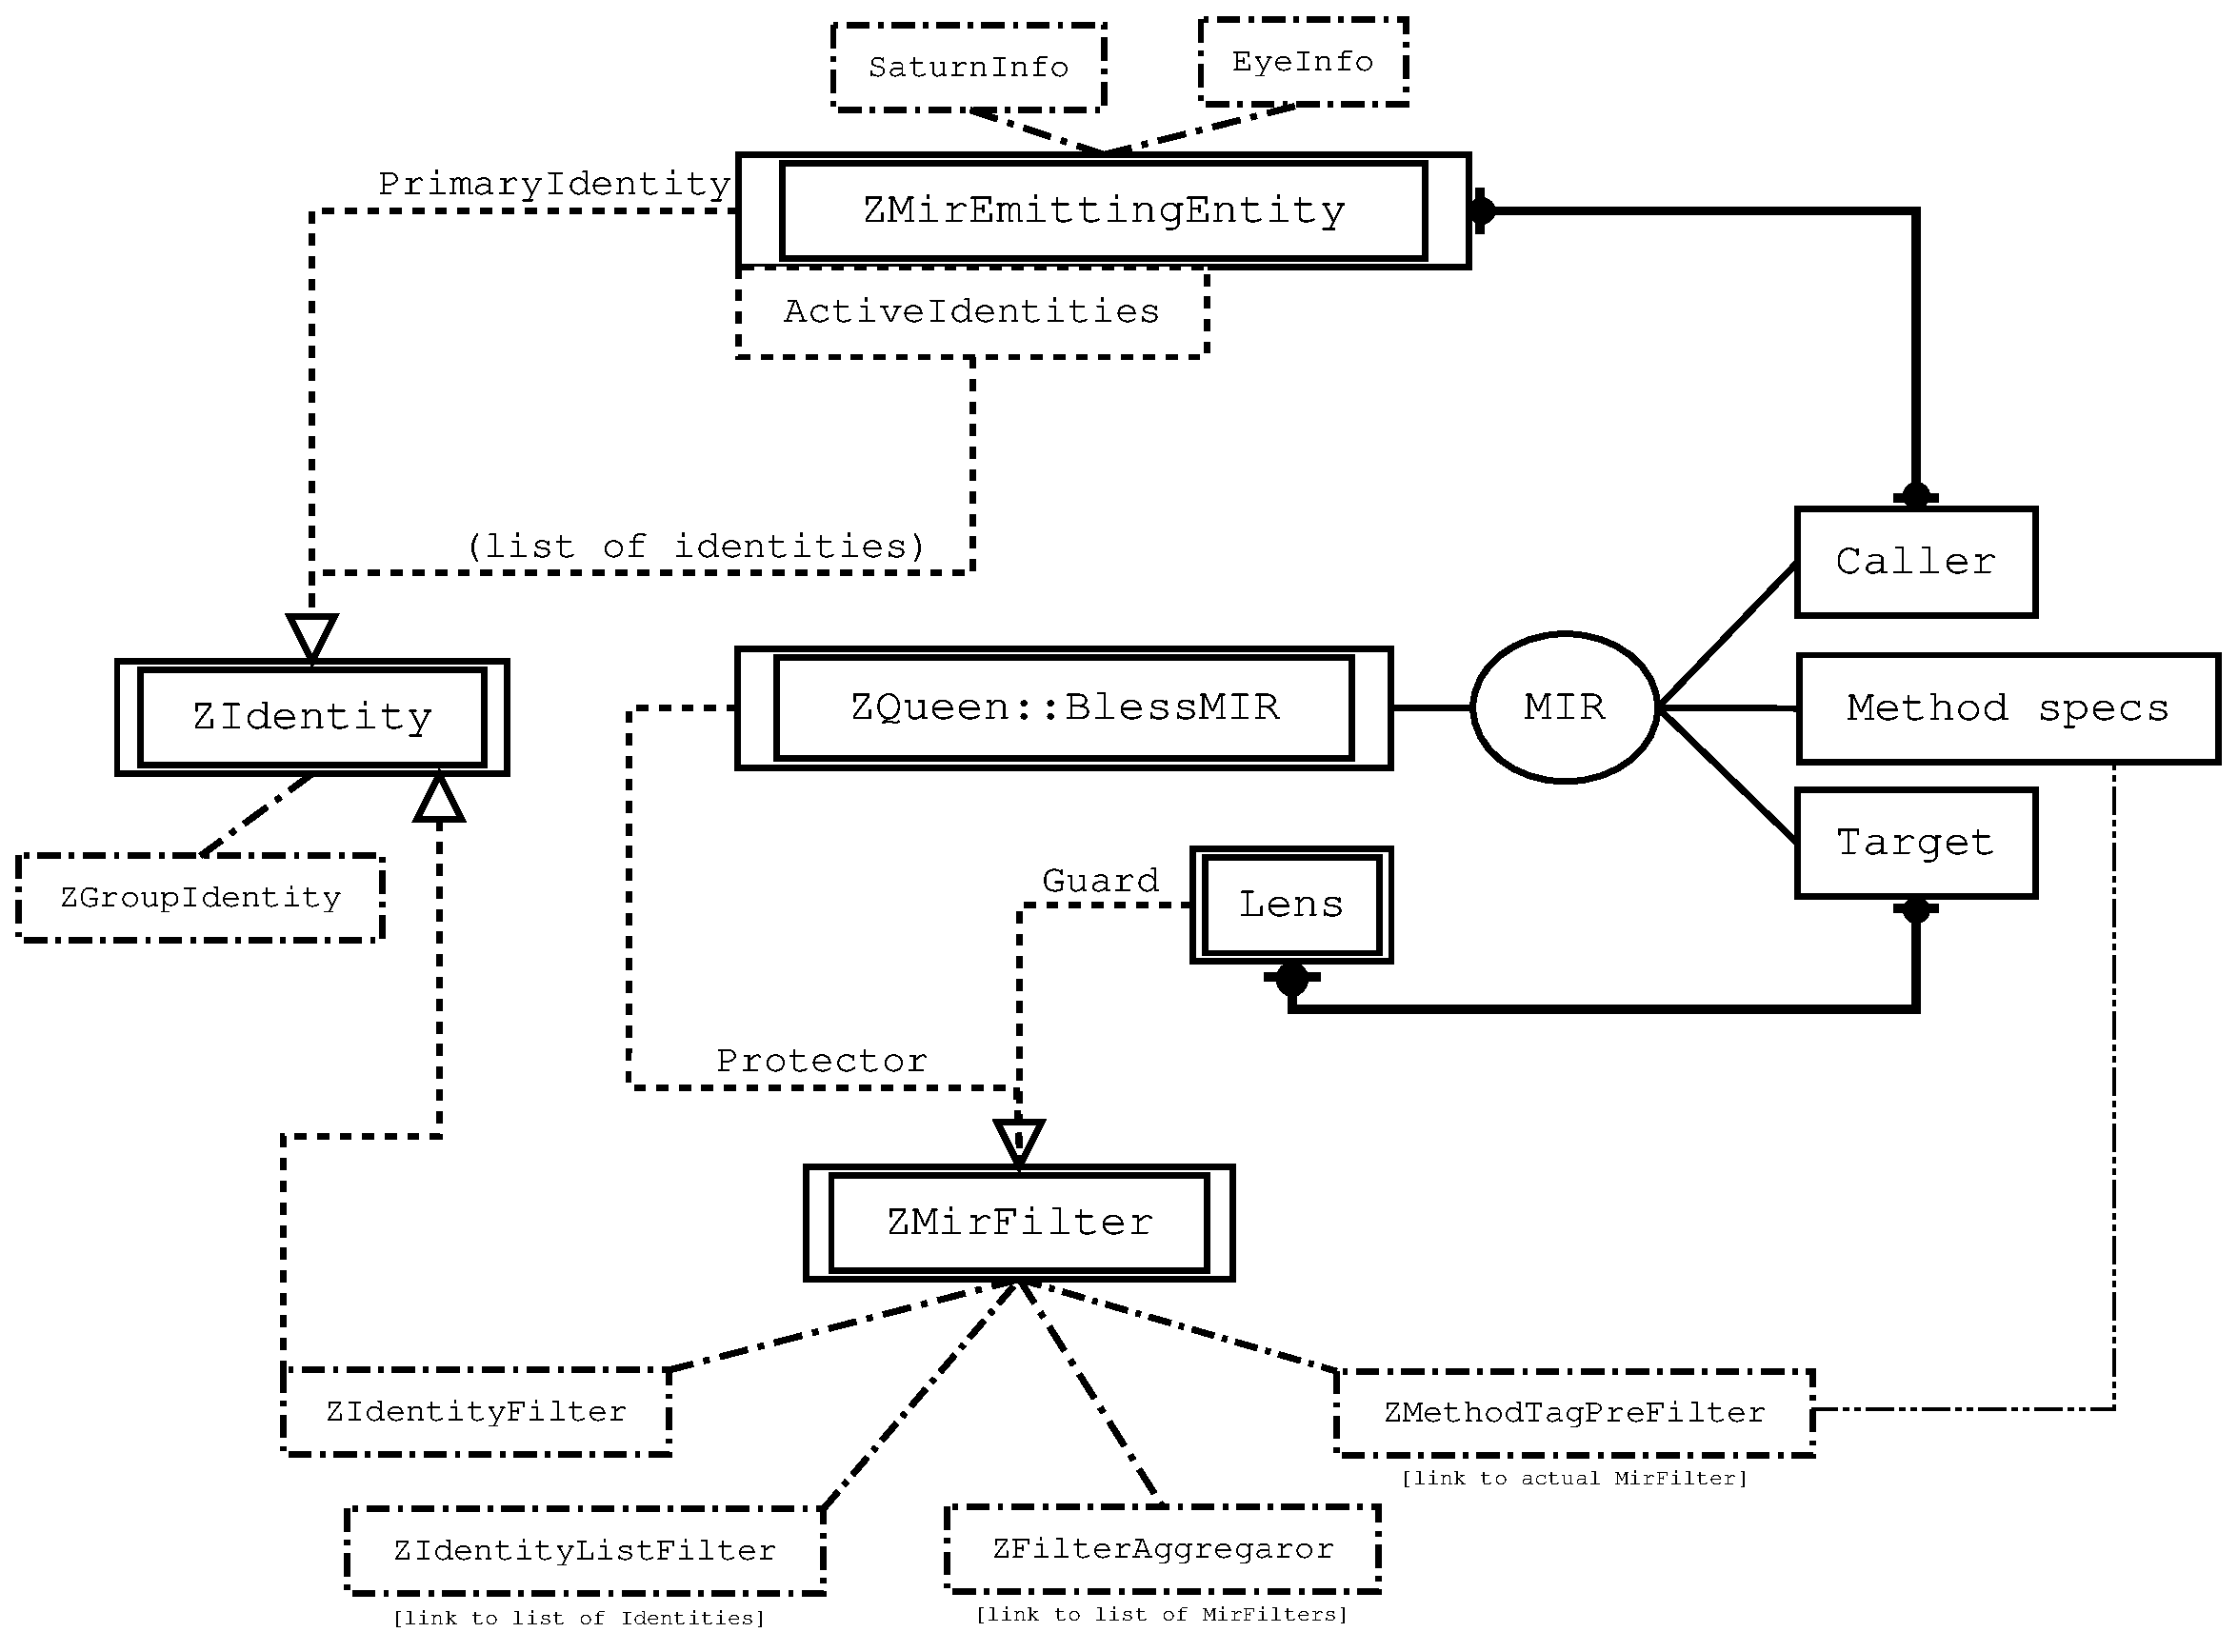
\includegraphics[height=\vsize]{\gledauthdir/aa_elements}}

\newpage
%%%%%%%%%%%%%%%%%%%%%%%%%%%%%%%%%%%%%%%%%%%%%%%%%%%%%%%%%%%%%%%%%%%%%%%%
% User threads \& GUI

\textbf{\LARGE User-Thread support:} base-glass
\texttt{\color{dblue}class Eventor :\ public Operator :\ public ZList}

provides traversal of \texttt{\color{dblue}Operator} tree in a dedicated thread
(via \texttt{\large\color{dblue}virtual void Operate(Operator::Arg*)}):\nl
\texttt{\large\color{dblue}Bool\_t bOpActive; Bool\_t bOpRecurse} \qq
can control tree traversal traversal\nl
all operations exception-throwing, with standard loop processing semantics:\nl
\hs6 {\large\color{dblue}\verb!enum Operator::Exc_e { OE_Done, OE_Continue, OE_Wait, OE_Stop, OE_Break };!}

\bl

{\LARGE Eventor: } modeled in accordance w/ HEP event-loop \qq but
this is a general model

\hbox to \hsize{
\vbox{\hsize=20cm

\texttt{\large\color{dblue}Int\_t mBeatsToDo} \qq%
  controls number of tree traversals to do (or events to process);\nl
  \qq\qq-1 means loop infinitely

\texttt{\large\color{dblue}Int\_t mInterBeatMS} \q%
  specifies the amount of sleep in between traversals\nl
  \qq\qq usefull for periodic tasks, {\color{dgreen}animation}

\texttt{\large\color{dblue} SaturnInfo* mHost; Bool\_t bMultix} \q
gives control of single/multi-host execution\nl
\bull if \texttt{Multix} on \,\qtoq run thread on all nodes (as well as suspend,
resume, stop)\nl
\bull if \texttt{Multix} off \qtoq use \texttt{Host} to determine
execution host\nl
\hs6 for expensive operations it pays-off to execute on one node and\nl
\hs6 broadcast results via a {\color{dblue}flared MIR}!

has methods to control the running state, \eg, {\large\texttt{Start(),
  Stop(), Suspend() \dots}}

provides timing of execution w/microsecond precision

\vss
}
\hfill
\includegraphics[width=6cm]{eventor_mtw}
}

\newpage
%%%%%%%%%%%%%%%%%%%%%%%%%%%%%%%%%%%%%%%%%%%%%%%%%%%%%%%%%%%%%%%%%%%%%%%%
% Eye etc

\textbf{\LARGE Lens-space observation, the \texttt{Eye} class and GUI elements:}
\bigskip

\hbox to \hsize{%
  \vbox{\hsize=17cm%
    Eyes connected to a local Saturn via TCP sockets\nl
    authenticated separately; represented by \texttt{EyeInfo} glass

    Eyes send {\color{dblue}MIRs} to Saturns to request a method invocation

    Receive {\color{dyellow}Rays} (change notifications events) from
    Saturn\nl
    dissolves Rays to all views of the affected lens\nl
    Eye holds \texttt{\large\color{dblue}hash\_map<ZGlass*, OptoStructs::ZGlassImage>}\nl
    which in turn contains
    \texttt{\large\color{dblue}list<OptoStructs::A\_View*>}\nl
    \texttt{\large\color{dblue}virtual void A\_View::AbsorbRay(Ray\&);}

    A nearly-optimal update performed (only on one class level)
  }
  \hss
  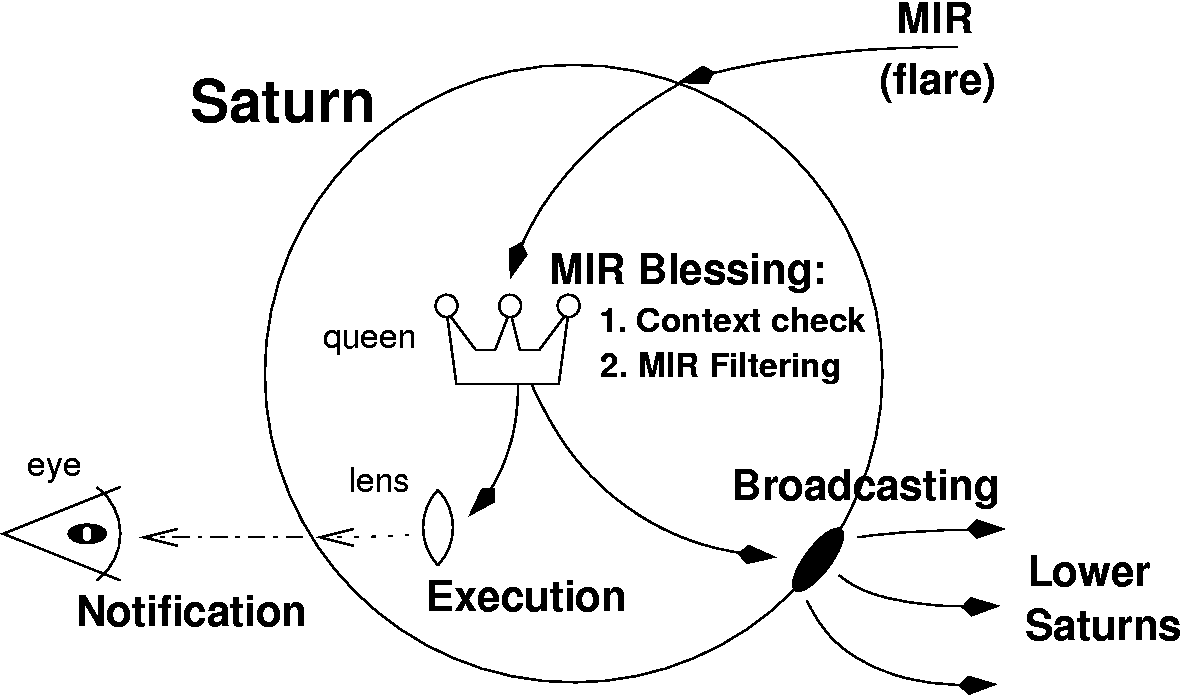
\includegraphics[width=11cm]{\gledihscmdir/figs/flare_exec}
}

\bigskip
\bl

{\LARGE Available GUI elements:} \hfill {\large\color{dgreen}(using FLTK
  -- the FastLightToolKit)}
\bigskip

{\color{dgreen}browser/editor of lens-graphs} (links and lists); optionally shows
custom data-view in a tabular format

{\color{dgreen}full-lens view} \qq\q\; allows editing/viewing of object-data \& execution
of methods wo/arguments

{\color{dgreen}method call widget} \q execution of methods with
{\color{dblue}lens}es and basic types as arguments\hfill%
(must add \texttt{\color{dblue}TObject}s)

{\color{dgreen}OpenGL viewer} \qq\; parallel Rnr class structure \qtoq
Rnr-state + decreases the weight of the base-class\nl
\hbox to 47.5mm{}RnrDriver aware of lens aggregation \qtoq lens
rendering proceeds on 7-levels\nl
\hbox to 47.5mm{}Rnr optimization\&adv. rnr-techniques, animation, impostors, etc.\nl

\smallskip

\gled build system produces {\color{dred}separate Core, GUI and GLRendering libraries}!

\newpage
%%%%%%%%%%%%%%%%%%%%%%%%%%%%%%%%%%%%%%%%%%%%%%%%%%%%%%%%%%%%%%%%%%%%%%%%
% ALICE stuff

\textbf{\LARGE (G)UI \& visualization of ALICE Distributed Analysis}
\bigskip

\textbf{AliEn / gLITE} as source of available \texttt{sites} +
file-location query

\begin{itemize}
\item display sites from a given partition (a subset of sites)
\item offer findEx interface: user enters query, \gled retrieves the
  info and shows files and their locations
\item user refines selection or appends another query or \dots
\item user starts-off the DA
\end{itemize}

\bl

\textbf{DataSet passed to PROOF} \qtoq performs the actual analysis

PROOF will be modified to (optionally, of course) also provide
progress reports with given time granularity

can be used to display/visualize progress

\bl

\textbf{web interface via CAROT}

user enters search-path, query and analysis macro \qtoq the results
appear on same web-page
 
CAROT, \gled and PROOF will use common \root classes to exchange
information describing the analysis progress

CAROT will offer a lightweigt UI, but can also ``record'' the session \qtoq
re-play w/\gled or just download

this recording can also be used:\nl
for monitoring/analysis of greed's performance \& responsivness\nl
by administrators to snoop on users

\newpage
%%%%%%%%%%%%%%%%%%%%%%%%%%%%%%%%%%%%%%%%%%%%%%%%%%%%%%%%%%%%%%%%%%%%%%%%
% hierarchy

\Huge
\hbox to 1mm{}
\vfill

\centerline{The most basic concept of \gled is}

\vskip 1cm

\centerline{\color{dblue}HIERARCHY}

\vskip 1cm

\centerline{with cross-links and exceptions}

\vfill
\hbox to 1mm{}
%%%%%%%%%%%%%%%%%%%%%%%%%%%%%%%%%%%%%%%%%%%%%%%%%%
\end{document}
%%%%%%%%%%%%%%%%%%%%%%%%%%%%%%%%%%%%%%%%%%%%%%%%%%
